\section{Used Models and Images}
\label{sec:data}
% vortrainierte Neural Networks erklären/erwähnen
% alle basieren auf der Image Database "ImageNet"
For the upcoming experiments in section \ref{sec:evaluation} we need to decide which network model we use and which images are feasible as source or \emph{guide image}.
As classification network we chose to use \emph{ResNet}\cite{he2016deep}, shorthand for \emph{Residual Network}, because it is the current state of the art providing the lowest error rate and hence performs best.\cite{cnnComparison}
It offers three variations differing in the layer amount, namely 50, 101, 152.
Due to performance reasons, see section \ref{sec:performance}, we decided to use the \emph{ResNet50}.
To apply the dream we use a modified version of the original \textit{Google Deep Dream} code\cite{deep-dream-github} for the neural network framework \textit{Caffe}\cite{jia2014caffe}.

By analyzing various existing dreamed images, we came to the conclusion that images with a lot of varying objects offering different features might lead to more interesting results.
Hence we were looking for images containing: 
\begin{itemize}
	\item a landscape with varying vegetation
	\item houses
	\item water because it offers a lot of noise to act upon
	\item clouds because of the real-life relatability mentioned in section \ref{sec:visual-aspects}
\end{itemize}

To find images with these properties we used \emph{Flickr} because it allows to search for images that are licensed under the \emph{creative commons}.
Figure \ref{fig:imgbeestemarkt} is an image of the Beestenmarkt in Leiden and offers three of the wanted features: water, clouds and buildings.
In addition to that a few people are also present in the picture who might be transformed as well.
The second image, visible in figure \ref{fig:imglandscape}, is a closeup of some vegetation on a field offering a lot of small distinctive features.
It contains two of the features we are looking for, namely a landscape with varying vegetation and houses.
It is also advantageous that the grass is made up of different colors.



\begin{figure}[H]
	\minipage{0.49\textwidth}
	\centering
	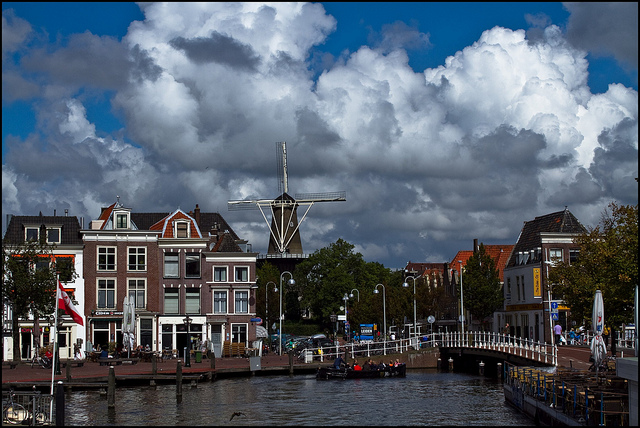
\includegraphics[width=1\linewidth]{img/beestemarkt.jpg}
	\caption{First source image displaying the Beestenmarkt in Leiden.\cite{imgbeestemarkt}}
	\label{fig:imgbeestemarkt}
	\endminipage\hfill
	\minipage{0.49\textwidth}
	\centering
	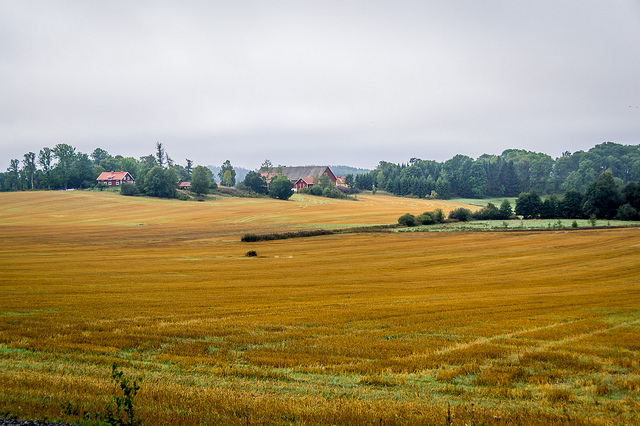
\includegraphics[width=1\linewidth]{img/landscape.jpg}
	\caption{Second source image portraying a landscape with small houses and trees.\cite{imglandscape}}
	\label{fig:imglandscape}
	\endminipage\hfill
\end{figure}